Wie bereits in den psychoakustischen Annahmen beschrieben, ist die Diffusität des wahrgenommenen Schalls abhängig von der interauralen Dekorrelation der Ohrsignale. In einem vollkommen diffusen Schallfeld trifft der Schall aus allen Richtungen auf den Hörer, was stark dekorrelierte Ohrsignale zur Folge hat. Die Aufgabe des Dekorrelationsverfahrens in diesem Versuch, ist die Synthese der Diffussignale für die Lautsprecherwiedergabe. Das Dekorrelationsverfahren soll somit stark dekorrelierte Lautsprechersignale zur Verfügung stellen, um die Diffusität des erzeugten Schallfeldes zu gewährleisten, ohne Artefakte zu erzeugen.

Es wurden drei Dekorrelationsverfahren verglichen. \textit{Random Phase} ist die originale DirAC Methode und weiters wurde ein \textit{Feedback Delay Network} und \textit{Widening} verwendet, die beide als Plugin verfügbar waren.

\paragraph{Random Phase}
Bei diesem Verfahren wird das Diffussignal mit weißem Rauschen gefaltet. Dabei ändert sich das Betragsspektrum des Signals nicht, aber das Phasenspektrum wird zufällig. Damit die Lautsprechersignale dekorreliert sind, müssen sich die Rauschsignale für die Faltung unterscheiden. Um Artefakte zu vermeiden, werden in drei Frequenzbereichen exponentiell abfallende Rauschsignale mit unterschiedlichen Zeitkonstanten verwendet.

\paragraph{Feedback Delay Network}

In Abbildung ~\ref{fig:fdn} ist ein Feedback Delay Network (FDN) für 3 Signale zu sehen. Die Eingangssignale werden mit Delays zeitverzögert, deren Länge $M_i$ Primzahlverhältnisse haben sollen, um ausgeprägte Resonanzen zu vermeiden.

\begin{figure}[!ht]
  \centering
  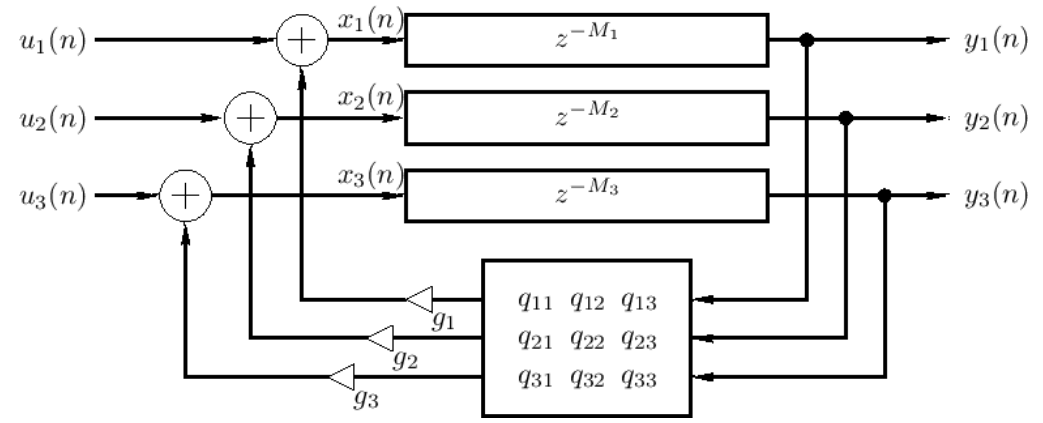
\includegraphics[width=0.9\textwidth]{dekorrelation/pic/FDN_smith.png}
  \caption{Feedback Delay Network für 3 Signale (Smith)}
  \label{fig:fdn}
\end{figure}


Die verzögerten Eingangssignale werden zurückgeführt über eine Mischungsmatrix

$Q = \begin{pmatrix} q_{11} & q_{12} & q_{13} \\
                     q_{21} & q_{22} & q_{23} \\
                     q_{31} & q_{32} & q_{33} \\
     \end{pmatrix}$.

Die gemischten Signale werden noch mit den Verstärkungsfaktoren $g_i$ multipliziert und schließlich zu den Eingangssignalen addiert. Das Verhalten des FDN hängt maßgeblich von den Delay-Längen $M_i$ und von den Eigenschaften der Mischungsmatrix $Q$ ab.

Prinzipiell eignet sich ein FDN gut zur Simulation von späten Reflexionen. In diesem Versuch wurden sehr kurze Nachhallzeiten verwendet, um die Diffusität der Signale zu erhöhen, ohne den Eindruck eines zusätzlichen Raums durch das FDN zu verursachen.

\paragraph{Widening}
Der Widening-Effekt wird durch frequenzabhängiges Panning um die Panning-Richtung erzeugt \cite{ambi-book}. Dabei werden aufeinanderfolgende Frequenzanteile in der Richtung leicht versetzt. Es kommt auch zu einer verschmierung der zeitlichen Feinstruktur des Signals. Dieser Effekt wird als Erhöhung der Distanz und Diffusität wahrgenommen und kann zur Simulation von frühen lateralen Reflexionen verwendet werden.
